\chapter{Introducción}
\label{ch:CH01}
\ihead[]{Cap\'itulo 1: Introducción}
%%%%%%%%%%%%%%%%%%%%%%%%%%%%%%%%%%%%%%%%%%
En este capítulo se explica y detalla la problemática de esta tesis, así como sus objetivos y alcances. Asimismo, se especificará la metodología de diseño a usar que se emplea para alcanzar los objetivos planteados.
%%%%%%%
\section{Problemática y Motivación}
\label{sec:CH01_Problematica}

En el ámbito universitario, el déficit de atención es un problema creciente que afecta el desempeño académico de los estudiantes. Una de las principales causas es la constante exposición a la sobrecarga de información, especialmente a través de internet y redes sociales, donde predomina la información en formato breve y la falta de estrategias de aprendizaje efectivas. Esto se ve reflejado en un estudio realizado a universitarios egipcios \autocite{safy2024effect}, donde se encontró que el uso promedio en dichas plataformas es entre 3 y 6 horas, identificándose como uno de las principales fuentes de distracción en estudiantes universitarios. Además, correlaciona la dificultad para gestionar grandes volúmenes de datos, debido a la ausencia de estrategias eficaces para manejar la distracción, como  es el caso de la técnica Pomodoro, la cual ayuda a organizar el tiempo de estudio de manera estructurada.\\

Uno de los estudios, que evidencia dificultad para mantener la concentración en el proceso de aprendizaje, es el análisis realizado a 122 estudiantes del Instituto Tecnológico Superior de Libres ubicado en México. Según \textcite{baez2021analisis}, en base a las frecuencias de ondas cerebrales, los resultados del estudio demostró los distintos niveles de concentración que presentan los estudiantes (ver Tabla ~\ref{tab:niveles_concentracion}). En donde se menciona que solo el 24\% indicó tener una concentración profunda o estado de calma como se muestra en la Figura~\ref{fig:niveles_concentracion}, mientras que 5\% presentan una mente activa donde la concentración fluctúa, el 29\% presenta una mente medianamente activa, el 32\% tiene una mente neutral, pero sin enfoque profundo y el 10\% restante presenta una mente medianamente neutral.

% \caption{Distribución de los niveles de concentración en los estudiantes}
%\captionof{table}{Tipos de Niveles de Concentración}
 
\begin{table}[H]
    \centering
    \begin{minipage}{0.4\textwidth}
        \centering
        \begin{figure}[H]
            \centering
            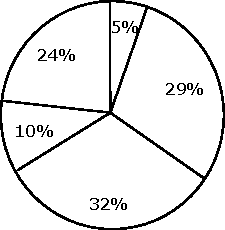
\includegraphics[width=0.7\linewidth]{CHPTRS/CH01_INT/Fig/01_niveles_concentracion.pdf}
            \caption{Distribución de los niveles de concentración en los estudiantes.}
            \label{fig:niveles_concentracion}
        \end{figure}
    \end{minipage}
    \hfill
    \begin{minipage}{0.55\textwidth}
        \centering
        \caption{Tipos de niveles de concentración en los estudiantes.}
            \label{tab:niveles_concentracion}
          
        \begin{table}[H]
            \centering
            {\small  
            \begin{tblr}{
              colspec = {Q[c,m]Q[l,m]},
              column{1}={0.3\textwidth},
              column{2}={0.6\textwidth},
              hlines,
              vlines,
              hline{1,7} = {-}{0.08em},
            }
            \textbf{Nivel de Concentración} & \textbf{Explicación} \\
            Mente Activa            & Indica una mente totalmente distraída con atención fluctuante.                                                             \\
            Medianamente Activa     & Indica una mente distraída pero la atención fluctúa.                                                                       \\
            Neutral                 & Indica que la atención se encuentra cuando hay total reposo, la atención no fluctúa pero no hay enfoque profundo presente. \\
            {Medianamente\\Neutral} & Indica que la atención se encuentra cuando hay reposos, sin atención fluctuante, sin enfoque profundo presente.            \\
            {Profunda o\\Calma}     & Indica los momentos en los que los estudiantes están completamente concentrados.                                           
            \end{tblr}
            }
        \end{table}
    \end{minipage}
    
    
    \caption*{\textit{Nota: Información tomada de Análisis del Estrés y Nivel de Concentración de Estudiantes Universitarios Durante Periodos de Exámenes de \textcite{baez2021analisis}.}}
  
\end{table}



%%%%%%
Por otro lado, en un estudio realizado a estudiantes universitarios de Barranquilla \autocite{contreras}, 55\% de los 32 analizados mencionaron que un factor clave asociado a su fracaso académico son los problemas de atención y concentración. Esta percepción evidencia que los propios estudiantes reconocen la falta de atención como una dificultad significativa en su proceso de aprendizaje, reforzando la urgencia de abordar esta problemática desde el ámbito educativo.\\

	Asimismo, si bien este trabajo no esta enfocado en el trastorno de déficit de Atención (TDAH), es importante mencionar que, en Latinoamérica, 36 millones de personas se ven afectadas por dicho trastorno, y solo una cuarta parte recibe una intervención. En el caso de Perú, se estima que entre el 5\% y el 10\% de la población padece de TDAH, lo que afecta el desarrollo integral y la calidad de vida de aquellos que lo padecen \autocite{davila2023trastorno}. \\
    
De lo mencionado, este trabajo se ve motivado ha explorar, seleccionar y diseñar estrategias, herramientas y tecnologías que permitan mejorar la capacidad de atención de los estudiantes universitarios. Esto se debe a la capacidad de los dispositivos tecnológicos para enriquecer el aprendizaje en el sector educativo. \autocite{wearable}. Es importante destacar que esta tecnología no solo debe diagnosticar la falta de atención, sino que debe brindar retroalimentación para fomentar la autorregulación de la atención del estudiante y desarrollo de hábitos de estudio.


%%%%%%%%%%%%%%%%%%
 
    

% NOTA: Para usar una figura al lado de otra se puede usar el paquete \tabularx, la idea es:
%       COL-1     COL-2
%   |----------*-----------*
%   | fig.A    | fig.B     |  FILA-1
%   |----------*-----------*
%   |caption a | caption b |  FILA-2
%   |label a   | label b   |
%   |----------*-----------*
%   |Nota a    | Nota b    |  FILA-3
%   |----------*-----------*
%   caption figura en general
%   label Figura en general.
%\begin{figure}[!ht]
 %   \begin{tabularx}{\linewidth}{*{2}{>{\centering\arraybackslash}X}}
  %      % FILA-1, COL-1.
   %     \begin{subfigure}[t]{0.45\textwidth}
   %         \centering
   %         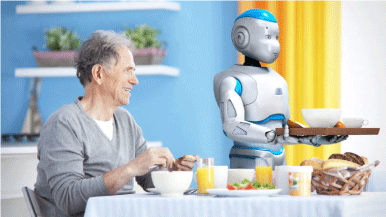
\includegraphics[width=.9\linewidth]{CHPTRS/CH01_INT/Fig/02a_Maxon-Romeo.png}
   %         %\label{fig:romeo} %LABEL ESTA DESPUES
    %    \end{subfigure}
    %    & %Nueva Columna, es decir: % FILA-1, COL-2
    %    \begin{subfigure}[t]{0.45\textwidth}
     %%      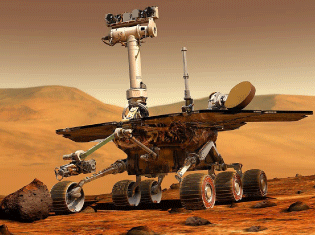
\includegraphics[width=.68\linewidth]{CHPTRS/CH01_INT/Fig/02b_Perseverance.png}
       % \end{subfigure}
%        \\ %Nueva Fila, es decir: % FILA-2, COL-1
 %       \begin{subfigure}[t]{0.8\linewidth}
  %          \caption{Imagen referencial del robot humanoide Romeo}
  %          \label{fig:romeo}
  %      \end{subfigure} 
  %      & %Nueva Columna, es decir: % FILA-2, COL-2
  %      \begin{subfigure}[t]{0.8\linewidth}
   %         \caption{Imagen referencial del rover \textit{Perseverance}}
   %         \label{fig:perseverance}
    %    \end{subfigure}
    %    \\ %Nueva Fila, es decir: % FILA-3, COL-1
     %   \begin{subfigure}[t]{\linewidth}
     %       \caption*{\textit{Nota: Figura tomada de la página oficial de \linebreak\textcite{ej-03-cita-pag-web}}}
      %  \end{subfigure} 
       % & %Nueva Columna, es decir: % FILA-3, COL-2
       % \begin{subfigure}[t]{\linewidth}
            %\caption*{\textit{Nota: Figura tomada de la página oficial de \linebreak\textcite{ej-03-cita-pag-web}}}
  %      \end{subfigure}
  %  \end{tabularx}
  %  \caption{Descripción General de las figuras presentadas}
  %  \label{fig:figuraEnGeneral}
%\end{figure}
%





\section{Propuesta de solución}
\label{sec:CH01_Propuesta}
El asistente que se propone para ayudar a mejorar la capacidad de concentración de los estudiantes universitarios estará compuesto por un sistema de adquisición de señales para monitorear indicadores fisiológicos relacionados a la atención o distracción del usuario. Este tendrá un diseño físico que será compacto, portátil y resistente a golpes, agua y polvo para que los alumnos sean capaces de utilizarla en distintos entornos académicos estándar como aulas de clase, bibliotecas o escritorios , basándose en estándares de protección como el IP67, cuya viabilidad será evaluada durante el diseño de la carcasa. Utilizando un algoritmo de pérdidas de enfoque y luego de detectar la distracción, el asistente brindará retroalimentación inmediata a través de una alerta, buscando reconectar al estudiante con su actividad académica. Finalmente, el sistema será flexible, permitiendo configurar el tiempo de estudio y los periodos de descanso, adaptándose a las necesidades del estudiante.
    
    \section{Objetivos}
    \label{sec:CH01_Objetivos}
        En esta sección, se mencionarán los  objetivos en esta tesis.
        
        \subsection{Objetivo Principal de la Tesis}
        
           
    
                Diseñar un asistente que ayude a mejorar tanto la concentración como reducir el déficit de atención en estudiantes universitarios que brinde retroalimentación al usuario en caso de distracción.
                
                
            
            \subsection{Objetivos específicos de la Tesis}
        \begin{itemize}
            \item Analizar la problemática de la falta  de concentración en entornos de aprendizaje mediante la investigación y revisión de dispositivos y tecnologías que permitan detectar y mejorar la atención de los estudiantes.
            %\item Indagar la problemática que enfrenta la tesis.
             %\item Analizar dispositivos actuales que ayudan a mejorar la concentración en entornos de aprendizaje.
            %\item Analizar y presentar tecnología que permite detectar falta de concentración en estudiantes.
            \item Determinar los requerimientos del asistente para poder determinar el concepto de solución óptimo para el desarrollo del proyecto.
            %\item Realizar diferentes alternativas de solución para el diseño del asistente.
           % \item Elegir el concepto solución óptimo para el desarrollo del proyecto.
           \item Realizar el diseño mecánico del asistente, incluyendo planos mecánicos, cálculos relevantes y modelado 3D del asistente.
            \item Diseñar el circuito eléctrico del sistema y la selección de componentes adecuada para el asistente.
            \item Diseñar el sistema de control e interfaz del asistente.
            %\item Elaborar los planos mecánicos del asistente.
            %\item Elaborar los planos electrónicos del asistente.
            %\item Elaborar el sistema de control del asistente.
            %\item Elaborar la interfaz del asistente.
            
            \item Validar la mejora de concentración a través de simulaciones realizadas a partir de los componentes seleccionadaos, validando su funcionamiento.
            \item Detallar los costos que conlleva la fabricación del proyecto para garantizar un bajo costo en el desarrollo del asistente.
            \end{itemize}
%%%%%%%%%%%%%%%%%%%%%% OBJETIVOS TFC1            
    %    \subsection{Objetivo Principal del Curso}
              
    
    %           Realizar el diseño conceptual de un asistente que ayude a mejorar la concentración y reducir el déficit de atención en estudiantes universitarios.
                
           
            
     %       \subsection{Objetivos específicos del Curso}
      %  \begin{itemize}
            
       %     \item Detallar la problemática, propuesta de solución y objetivos de la temática presentada.
        %     \item Analizar dispositivos actuales que ayudan a mejorar la concentración en entornos de aprendizaje.
         %   \item Definir los requerimientos técnicos y funcionales del asistente.
           % \item Elaborar la estructura de funciones del asistente.
          %  \item Realizar las matrices morfológicas basadas en los subsistemas planteados
            %\item Realizar diferentes alternativas de solución para el diseño del asistente
            %\item Evaluar y seleccionar el concepto solución óptimo mediante criterios técnicos y económicos verificando que se cumplan todos los requerimientos
           
            %\end{itemize}
%%%%%%%%%%%%%%% OBJETIVOS TFC1
            
    \section{Alcance}
    \label{sec:Alcance}
     El asistente será diseñado para ser usado en entornos académicos como bibliotecas, aulas o espacios de estudio individual, priorizando un diseño portátil y económico. La solución no está especialmente dirigida a personas con diagnósticos clínicos como el \ac{TDAH} ni mucho menos reemplaza intervenciones terapéuticas o médicas. Se espera que el asistente alcance un nivel de madurez tecnológica TRL4 \autocite{ibanez2014niveles} y en caso de no poder implementar alguna parte de un subsistema, se optará por validar su funcionamiento a través de simulaciones funcionales que permitan evaluar su desempeño teórico.
%%%
    
    \section{Metodología}
  

    	La metodología que se utilizará para este trabajo es la VDI 2221 \autocite{jansch2006development}, la cual permite abordar el problema y solucionarlo desde un punto de vista mecatrónico, ya que permite estructurar el proceso de diseño desde la comprensión del problema hasta la definición detallada de la solución. La VDI 2221 se basa en un enfoque en cascada que consta de varias fases: análisis de requerimientos, definición de funciones, generación de soluciones conceptuales, diseño preliminar, y diseño detallado (ver Figura~\ref{fig:vdi2221}).\\
        
        Complementariamente, se considerará la metodología VDI 2206 \autocite{ej-06-cita-norma-vdi2206} para el desarrollo de sistemas mecatrónicos. Esta, basada en el modelo en V (ver Figura ~\ref{fig:vdi2206}) que permite el desarrollo en paralelo de los subsistemas mecánico, eléctrico y de \ac{SW}. En el lado izquierdo del modelo ingresan las exigencias del sistema, se desarrolla la descomposición del proyecto en especificación funcional  que dan lugar a los dominios del proyecto. En el lado derecho se realiza la integración del sistemas, generando como salida el producto completo. Para ello, el modelo plantea un aseguramiento de propiedades entre ambos lados a través de simulaciones o pruebas que garantizan que los requisitos definidos al inicio. De esta manera, la metodología VDI 2206 permite mantener la coherencia funcional y validar progresivamente los objetivos del sistema.\\
        
        Asimismo, al momento de realizar los análisis técnicos y económicos se utilizará la metodología VDI 2225 siguiendo el ejemplo práctico de  \textcite{sandoval2025conceptual}, ya que este establece un método de decisión optimizado al mínimo coste a través de una evaluación cuantitativa de criterios técnicos y económicos. De esta manera, se podrá tener certeza que se ha elegido el diseño conceptual más optimo. \\

       Según lo mencionado anteriormente, se organizará el documento de la siguiente manera: El \hyperref[ch:CH02-Estado-del-Arte]{segundo capítulo} se centrará en realizar un marco teórico sobre las variables fisiológicas relacionadas con la atención, además de describir la tecnología existente que busca hacer frente a la problemática. El \hyperref[ch:CH03-Diseno-Conceptual]{tercer capítulo} está enfocado en el diseño conceptual del asistente, es decir, requerimientos del asistente, estructura de funciones, matriz morfológica y los conceptos solución junto con sus análisis técnico-económicos. El cuarto capítulo se centrará en el diseño detallado, es decir, se presentará el diseño mecánico, electrónico y de software del asistente. En el quinto capítulo se realizará la validación y se mostraran los resultados en base a los requerimientos mediante simulaciones o pruebas experimentales. Finalmente, en el sexto capítulo, se brindarán las conclusiones y recomendaciones sobre el trabajo realizado.

\begin{landscape}

       
\begin{figure}[H]
    \centering
    \begin{subfigure}[b]{0.6\textwidth}
     \label{sec:CH01_Metodologia}
    
\includegraphics[width=\textwidth]{CHPTRS/CH01_INT/Fig/03_VDI2221.PNG.pdf}
    \caption{Proceso Generalizado de Desarrollo y Diseño VDI 2221}
    \caption*{\textit{Nota: Figura adaptada de \autocite{ej-08-cita-norma-vdi2221}}}
    \label{fig:vdi2221}
    \end{subfigure}
    \hfill
    \begin{subfigure}[b]{0.7\textwidth}
          \centering
           \label{sec:CH01_Metodologia}
    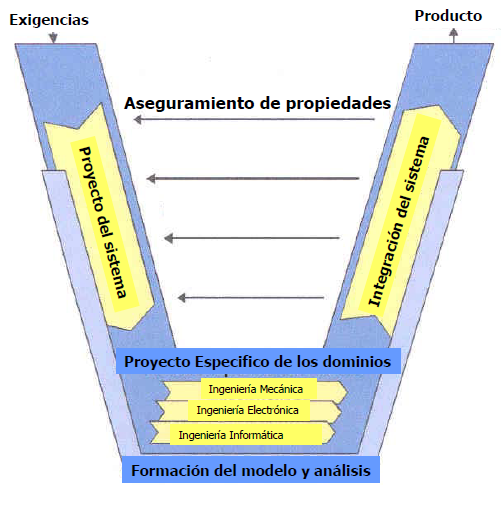
\includegraphics[width=\textwidth]{CHPTRS/CH01_INT/Fig/04_VDI2206.PNG}
    \caption{Modelo V de la metología VDI 2206}
    \caption*{\textit{Nota: Figura adaptada de \autocite{ej-06-cita-norma-vdi2206}}}
    \label{fig:vdi2206}  
    \end{subfigure}
\end{figure}  

\end{landscape}


        
    %En el desarrollo de este trabajo de investigación se usará la metodología VDI %2221 y VDI 2206, ambas desarrolladas por ... \autocite{ej-06-cita-norma-%vdi2206}. La primera metodología \lipsum[1] \ref{fig:vdi2221}. Ver %\lipsum[2]\autocite{ej-08-cita-norma-vdi2221}.
    
  
    
    
     
    
    